\documentclass[12pt]{article}

\usepackage[]{graphicx}
\usepackage[]{color}
\usepackage{alltt}
\usepackage{verbatim}
\usepackage{listings}
\usepackage{graphicx}
\usepackage{apacite}
\usepackage[acronym,nomain,nonumberlist]{glossaries}
\usepackage{fixltx2e}
\usepackage{graphicx}
\usepackage{colortbl}
\usepackage{caption}
\captionsetup{justification=raggedright,singlelinecheck=false}

\newcommand{\mytitle}{Modular Software Architecture for a Remote Controlled Rasberry Pi Robot}
\newcommand{\myname}{Gjergji Shkurti}

\newcommand{\breakln}{\mbox{} \\}
\newcommand{\placeholder}[1]{\textcolor{red}{#1}}
\newcommand*{\captionsource}[2]{%
  \caption[{#1}]{%
    #1%
    \\\hspace{\linewidth}%
    \textbf{Source:} #2%
  }%
}

\usepackage[a4paper, width = 160mm, top = 35mm, bottom = 30mm,bindingoffset = 0mm]{geometry}
\usepackage[utf8]{inputenc}
\usepackage{ragged2e}
\usepackage{xcolor}
\usepackage[round, comma]{natbib}
\usepackage{fancyhdr}
\usepackage{gensymb}
\newcommand{\changefont}{%
    \fontsize{8}{11}\selectfont
}

\usepackage{hyperref}
\hypersetup{
  	pagebackref=true,
    hyperindex=true,
    colorlinks=true,
    breaklinks=true,
    urlcolor= black,
    linkcolor= black,
    bookmarks=true,
    bookmarksopen=false,
    filecolor=black,
    citecolor=black,
	urlbordercolor  = green,
    linkbordercolor=red
	}
\pagestyle{fancy}
\fancyhead{}
\fancyhead[R]{\changefont{\mytitle}}
\fancyfoot{}
\fancyfoot[R]{\thepage}
\setlength{\headheight}{14.5pt}
\setlength{\parindent}{0pt}
\interfootnotelinepenalty = 10000

% XML listing style -------------------------------------------------------------

\definecolor{maroon}{rgb}{0.5, 0.0, 0.0}
\definecolor{darkolivegreen}{rgb}{0.33, 0.42, 0.18}


\lstdefinelanguage{XML}
{
	basicstyle=\ttfamily\footnotesize,
	morestring=[b]",
	morecomment=[s]{<?}{?>},
	morecomment=[s]{<!--}{-->},
	commentstyle=\color{darkolivegreen},
	moredelim=[s][\color{black}]{>}{<},
	stringstyle=\color{blue},
	identifierstyle=\color{maroon},
	keywordstyle=\color{red},
	numbers=left,
	tabsize=2,
	frame=single,
	rulecolor=\color{black},
	breaklines=true,
	captionpos=b,
	morekeywords={xmlns, version, type, Algorithm, URI, Id, Target}% list your attributes here
}

% C++ listing style -------------------------------------------------------------

\definecolor{dkgreen}{rgb}{0,0.6,0}
\definecolor{dred}{rgb}{0.545,0,0}
\definecolor{dblue}{rgb}{0,0,0.545}
\definecolor{lgrey}{rgb}{0.9,0.9,0.9}
\definecolor{gray}{rgb}{0.4,0.4,0.4}
\definecolor{darkblue}{rgb}{0.0,0.0,0.6}

\lstdefinelanguage{cpp}{
      backgroundcolor=\color{lgrey},
      basicstyle=\footnotesize \ttfamily \color{black} \bfseries,
      breakatwhitespace=false,
      breaklines=true,
      captionpos=b,
      commentstyle=\color{dkgreen},
      deletekeywords={...},
      escapeinside={\%*}{*)},
      frame=single,
      language=C++,
      keywordstyle=\color{purple},
      morekeywords={BRIEFDescriptorConfig,string,TiXmlNode,DetectorDescriptorConfigContainer,istringstream,cerr,exit},
      identifierstyle=\color{black},
      stringstyle=\color{blue},
      numbers=left,
      numbersep=5pt,
      numberstyle=\tiny\color{black},
      rulecolor=\color{black},
      showspaces=false,
      showstringspaces=false,
      showtabs=false,
      stepnumber=1,
      tabsize=2,
      title=\lstname,
    }

% Python listing style ------------------------------------------------------------
\lstdefinestyle{python}{
    backgroundcolor=\color{backcolour},
    commentstyle=\color{codegreen},
    keywordstyle=\color{magenta},
    numberstyle=\tiny\color{codegray},
    stringstyle=\color{codepurple},
    basicstyle=\footnotesize,
    breakatwhitespace=false,
    breaklines=true,
    captionpos=b,
    keepspaces=true,
    numbers=left,
    numbersep=5pt,
    showspaces=false,
    showstringspaces=false,
    showtabs=false,
    tabsize=2
}

\IfFileExists{upquote.sty}{\usepackage{upquote}}{}
\AtBeginDocument{\hypersetup{pdfborder={0 0 1}}}
\begin{document}

% FRONT PAGE -------------------------------------------------------------------

\begin{titlepage}
	\begin{center}
		\rule{\textwidth}{1.5pt}
		\LARGE
		\textbf{\mytitle}
		\rule{\textwidth}{1.5pt}

        \vspace{0.5cm}

        \LARGE
		Documentation and Manual

        \vspace{0.7cm}

		\large
		\date

		\includegraphics[width=16cm]{../images/robot.png}

		\vfill

		\normalsize
		Developed by Gjergji Shkurti

	\end{center}
\end{titlepage}

\newpage
\tableofcontents
\newpage

\listoffigures
\listoftables
\newpage

\pagenumbering{arabic}

\section{Introduction}
\label{sec-intro}


\begin{figure}[tbh!]
	\centering
	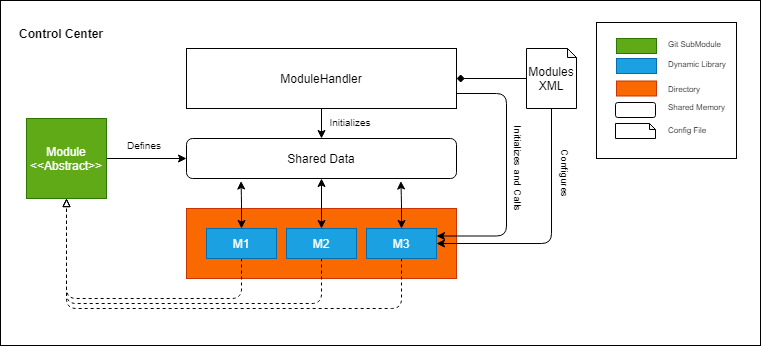
\includegraphics[width=16cm]{../images/overview.png}
	\caption{Overview}
	\label{fig:overview}
\end{figure}

\section{User Manual}
\label{sec-user-manual}

\subsection{Getting Started}
\label{subsec-getting-started}

\subsubsection{Installing Dependencies}
\label{subsubsec-installing-dependencies}

\subsubsection{Building the Control Center}
\label{subsubsec-building-control-center}

\subsection{Available Modules}
\label{subsec-available-modules}

\subsubsection{Controller}
\label{subsubsec-mod-controller}

\subsubsection{ZMQ Pipeline}
\label{subsubsec-mod-zmq-pipeline}

\subsubsection{Video Pipeline}
\label{subsubsec-mod-video-pipeline}

\subsubsection{Object Detector}
\label{subsubsec-mod-object-detector}

\subsubsection{Python Bridge}
\label{subsubsec-mod-py-bridge}

\subsection{External Python Modules}
\label{subsec-py-modules}

\subsubsection{Gesture Control}
\label{subsubsec-py-mod-gesture-control}

\subsubsection{Voice Control}
\label{subsubsec-py-mod-voice-control}

\subsection{Configuring and Running the Control Center}
\label{subsection-configure-and-run-control-center}

\section{Architecture}
\label{sec-architecture}

\subsection{Module Handler}
\label{subsec-module-handler}

\subsection{Module Configuration}
\label{subsec-module-config}

\subsection{Module Interface}
\label{subsec-module-interface}

\subsubsection{Initialization}
\label{subsubsec-module-init}

\subsubsection{Cycle Processing}
\label{subsubsec-module-cycle-step}

\subsubsection{Deinitialization}
\label{subsubsec-module-cycle-deinit}

\section{Developing Modules}
\label{sec-developing-new-modules}

\subsection{Module Template Generator}
\label{subsec-template-generator}

\subsection{Module Version Control}
\label{subsec-module-version-control}

\newpage


% ------------------------------------------------------------------------------
% BIBLIOGRAPHY -----------------------------------------------------------------
% ------------------------------------------------------------------------------

% \RaggedRight
% \bibliographystyle{apacite}
% \bibliography{References}

% \newpage
% \pagenumbering{Roman}
% \setcounter{page}{6}

\end{document}
